\section{Descripción del proceso de desarrollo}
\label{sec:desarrollo}

\subsection{Entorno y creación del proyecto}
El proyecto se crea con la herramienta de línea de comandos de Flutter. Se eligieron las plataformas Android y web (la web solo para revisar rápido el diseño); la aplicación no usa ningún paquete externo, únicamente el SDK.

\begin{lstlisting}[style=consola,caption={Comandos para preparar y verificar el proyecto.},captionpos=b]
flutter doctor                       # verifica SDK, Android Studio y emulador
flutter create --project-name matrlab --platforms android,web .
flutter pub get                      # descarga dependencias (solo el SDK)
flutter analyze                      # analisis estatico del codigo
flutter test                         # pruebas + generacion de capturas
flutter run                          # ejecuta en emulador o dispositivo
\end{lstlisting}

El archivo \texttt{pubspec.yaml} declara solamente \texttt{flutter} (y \texttt{flutter\_test} para las pruebas) y activa \texttt{uses-material-design} para disponer de los iconos Material (archivo \texttt{pubspec.yaml} del repositorio).

\subsection{Estructura del proyecto y arquitectura}
\begin{lstlisting}[style=consola,caption={Estructura de carpetas de \texttt{lib/} y \texttt{test/}.},captionpos=b]
lib/
  main.dart               # punto de entrada: runApp(MatrLabApp(...))
  app.dart                # MaterialApp, tema, decide Login o Shell
  models.dart             # Curso, GrupoLab, Horario, Matricula, Notificacion
  datos_demo.dart         # 5 cursos, 9 grupos, avisos iniciales
  estado.dart             # MatrLabState (reglas) + MatrLabScope (acceso)
  widgets/comunes.dart    # CupoBar, EstadoChip, StatTile, Aviso, ...
  screens/
    login_screen.dart  shell_screen.dart  cursos_screen.dart
    curso_detalle_screen.dart  grupo_detalle_screen.dart
    confirmacion_screen.dart  horario_screen.dart
    alertas_screen.dart  panel_screen.dart
test/
  matrlab_state_test.dart   # 17 pruebas de las reglas de negocio
  flujo_widget_test.dart    # flujo completo con widgets reales
  capturas_test.dart        # genera las 17 capturas del informe
\end{lstlisting}

\onefig{img/d_arquitectura.png}{0.85}{Arquitectura: las pantallas leen el estado a través de \texttt{MatrLabScope}; cuando el estado cambia llama a \texttt{notifyListeners()} y se reconstruyen las pantallas que dependen de él.}{fig:arq}

\subsection{Paso 1: el estado y las reglas de negocio}
Se separó la lógica de la interfaz. \texttt{MatrLabState} extiende \texttt{ChangeNotifier} y contiene los datos y las operaciones (\texttt{matricular}, \texttt{cancelarMatricula}, \texttt{unirseAListaEspera}, \texttt{ajustarCupos}, \texttt{conflictoCon}\ldots). \texttt{MatrLabScope} es un \texttt{InheritedNotifier}: un widget que coloca ese estado en lo alto del árbol y reconstruye automáticamente a todo widget que lo lea con \texttt{MatrLabScope.of(context)}. Así no se necesitó ningún paquete de gestión de estado. El método \texttt{matricular} aplica las reglas en orden: mismo curso, cruce de horario y cupo.

\extracto{lib/estado.dart}{116-134}{Regla de matrícula: valida, reserva el cupo y notifica (\texttt{lib/estado.dart}).}

\extracto{lib/estado.dart}{215-236}{Acceso al estado desde cualquier widget (\texttt{lib/estado.dart}).}


\subsection{Paso 2: widgets reutilizables}
Antes de las pantallas se construyeron los componentes que se repiten (sección~\ref{sec:catalogo}). \texttt{CupoBar} es el ejemplo más importante: una \texttt{Column} con una \texttt{Row} (texto a la izquierda, fracción a la derecha mediante \texttt{Spacer}) y una barra de progreso recortada con \texttt{ClipRRect}. El color se calcula a partir del estado del grupo.

\extracto{lib/widgets/comunes.dart}{83-133}{Componente CupoBar (\texttt{lib/widgets/comunes.dart}).}


\subsection{Paso 3: las pantallas}
Cada pantalla se programó siguiendo su mockup (sección~\ref{sec:mockups}). A continuación se muestra, para cada una, la captura de la aplicación, el fragmento clave y el funcionamiento de sus widgets.

\subsubsection{Inicio de sesión}
Un \texttt{Form} con una \texttt{GlobalKey} agrupa los dos \texttt{TextFormField}; al pulsar \emph{Ingresar} se llama a \texttt{validate()}, que ejecuta los \texttt{validator} y muestra los mensajes de error bajo cada campo. El \texttt{SegmentedButton<Rol>} cambia el rol, y con él la etiqueta y la regla del primer campo.

\extracto{lib/screens/login_screen.dart}{81-111}{Selector de rol y campo de código (\texttt{lib/screens/login\_screen.dart}).}

\duo{c01_login}{Pantalla inicial: logo, selector de rol, campos y botón.}{c02_login_validacion}{Al pulsar Ingresar con los campos vacíos: mensajes de validación.}{Inicio de sesión.}

\subsubsection{Estructura principal y lista de cursos}
\texttt{ShellScreen} es un \texttt{Scaffold} cuya barra de navegación depende del ancho disponible: un \texttt{LayoutBuilder} entrega las restricciones y, desde 600\,dp, se muestra un \texttt{NavigationRail} dentro de una \texttt{Row}; si no, una \texttt{NavigationBar} inferior. Las tres pestañas viven en un \texttt{IndexedStack}, que conserva el estado de cada una (por ejemplo, lo escrito en la búsqueda) al cambiar de pestaña.

\extracto{lib/screens/shell_screen.dart}{57-100}{Navegación adaptable (\texttt{lib/screens/shell\_screen.dart}).}


En \texttt{CursosScreen}, la cuadrícula se define con un \texttt{SliverGridDelegateWithMaxCrossAxisExtent}: cada tarjeta mide como máximo 480\,dp de ancho y 128\,dp de alto, y Flutter calcula cuántas columnas caben. En un teléfono resulta una sola columna; en una tableta, dos o más.

\extracto{lib/screens/cursos_screen.dart}{113-123}{Cuadrícula adaptable de cursos (\texttt{lib/screens/cursos\_screen.dart}).}

\duo{c03_cursos}{Pestaña Cursos: búsqueda, tres resúmenes, filtros y tarjetas.}{c04_cursos_busqueda}{Al escribir «datos» solo queda Base de Datos II.}{Lista de cursos con búsqueda.}

\subsubsection{Detalle de curso y de grupo}
La cabecera del curso es un \texttt{Stack}: el primer hijo (un \texttt{Padding} con el texto) queda debajo y el \texttt{Positioned} del icono decorativo se coloca en la esquina inferior derecha, parcialmente fuera; el \texttt{ClipRRect} recorta lo que sobresale. En el detalle del grupo, el botón de acción se decide según el estado: matricularse, cancelar, lista de espera o botón deshabilitado con la razón.

\extracto{lib/screens/curso_detalle_screen.dart}{27-75}{Cabecera con Stack y Positioned (\texttt{lib/screens/curso\_detalle\_screen.dart}).}

\extracto{lib/screens/grupo_detalle_screen.dart}{138-184}{Botón de acción según el estado del grupo (\texttt{lib/screens/grupo\_detalle\_screen.dart}).}

\trio{c05_curso_detalle}{Detalle del curso con sus dos grupos.}{c06_grupo_detalle}{Detalle del grupo: tabla de datos, cupos y botón fijo.}{c07_confirmar_sheet}{Hoja de confirmación sobre el detalle.}{Del curso al grupo y la confirmación de la matrícula.}

\subsubsection{Confirmación y horario}
Al confirmar, \texttt{matricular} reserva el cupo y la pantalla se reemplaza (\texttt{pushReplacement}) por la de éxito, de modo que el botón «atrás» no vuelva a la hoja. El horario semanal es una \texttt{Table}: la primera fila son los días y cada fila siguiente es una franja de dos horas; \texttt{\_grupoEn} busca si alguna matrícula ocupa esa celda y, de ser así, se pinta la sigla del curso.

\extracto{lib/screens/horario_screen.dart}{98-119}{Horario semanal con Table (\texttt{lib/screens/horario\_screen.dart}).}

\trio{c08_confirmacion}{Matrícula confirmada con el resumen.}{c09_horario}{Horario con PE (martes) y SI (miércoles).}{c10_horario_vacio}{Estado vacío: sin matrículas, con acción.}{Confirmación y horario semanal.}

\subsubsection{Casos especiales: cruce, grupo lleno y lista de espera}
Las reglas de negocio se ven en la interfaz. Con PE grupo A matriculado, el grupo A de Redes (mismo horario) muestra un aviso ámbar y el botón queda deshabilitado. En BD2 grupo B, que está lleno, el botón pasa a «Unirme a la lista de espera»; al unirse, el grupo aparece como \texttt{Chip} en Alertas.

\trio{c11_cruce_horario}{Cruce con PE grupo A: botón deshabilitado y aviso.}{c12_grupo_lleno}{Grupo sin cupos: lista de espera.}{c13_alertas_espera}{Alertas: lista de espera y notificaciones.}{Casos que resuelven las causas C4 y C5 del árbol de problemas.}

\subsubsection{Panel del administrador}
El panel usa un \texttt{GridView.count} dentro de un \texttt{ListView}. Como el \texttt{ListView} da altura ilimitada, el \texttt{GridView} necesita \texttt{shrinkWrap: true} y desactivar su propio scroll; sin eso Flutter lanzaría una excepción (tabla~\ref{tab:errores}).

\extracto{lib/screens/panel_screen.dart}{24-39}{Resúmenes del panel (\texttt{lib/screens/panel\_screen.dart}).}

\duo{c14_panel_admin}{Panel: resúmenes, grupo más saturado, ranking y gestión de cupos.}{c15_alertas_cupo_liberado}{Tras agregar un cupo a BD2 grupo B, el estudiante recibe «Se liberó un cupo».}{Causas C6 y C5: gestión de cupos y aviso al estudiante.}

\subsubsection{Diseño adaptable}
La misma aplicación, sin cambiar código, en una ventana de 1000\,$\times$\,640\,dp: aparece el riel de navegación, el contenido se centra con ancho máximo y la lista de cursos pasa a dos columnas.

\ancha{c16_tablet_cursos}{Cursos en tableta: \texttt{NavigationRail} y cuadrícula de dos columnas.}{fig:tab1}
\ancha{c17_tablet_horario}{Horario en tableta: el contenido se limita a 720\,dp y se centra.}{fig:tab2}

\subsection{Del mockup a la aplicación}
La figura~\ref{fig:comp} compara tres mockups con las pantallas implementadas. Las diferencias son de detalle (tipografía real, iconos reales en lugar de bloques); la estructura de cada pantalla se conserva.

\begin{figure}[!htbp]\centering
\begin{subfigure}[t]{0.17\textwidth}\centering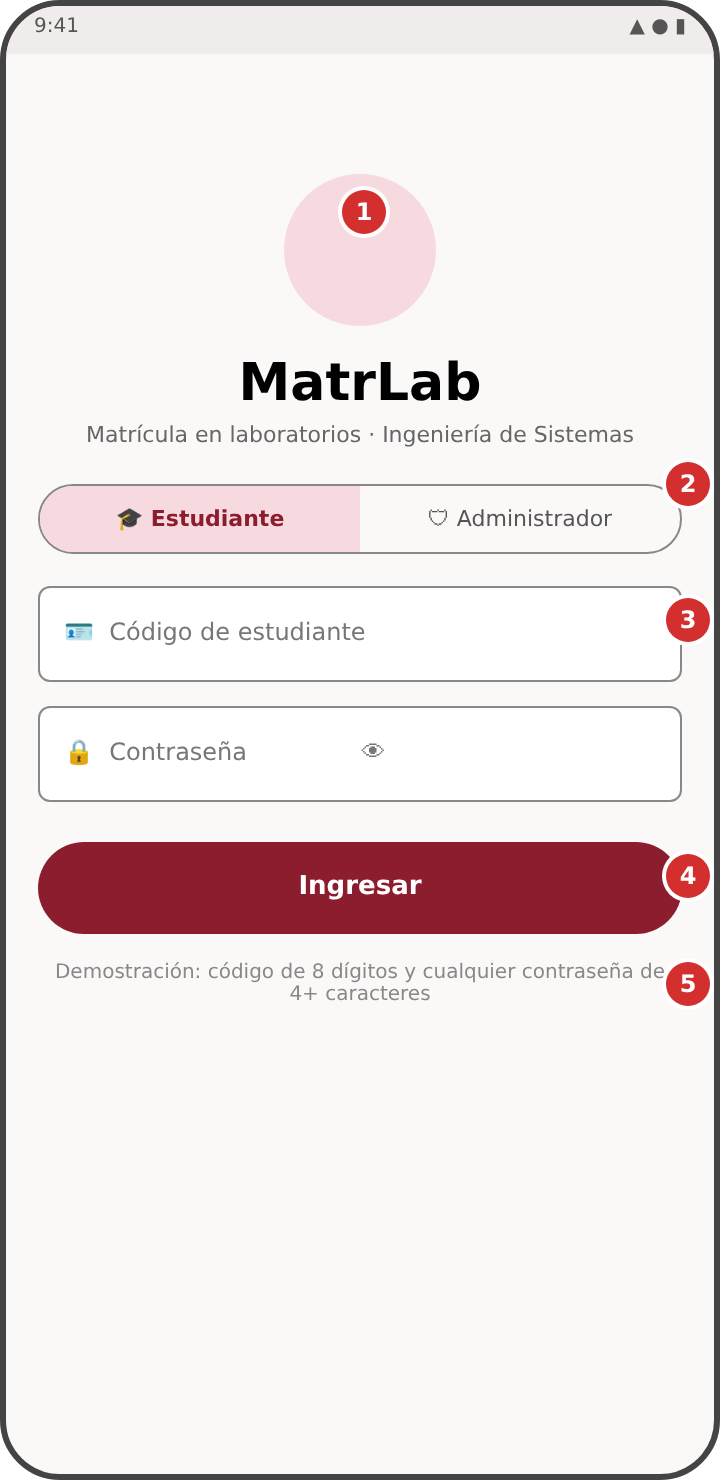
\includegraphics[width=\linewidth]{img/m01_login.png}\caption{Mockup}\end{subfigure}
\begin{subfigure}[t]{0.17\textwidth}\centering\capt{c01_login}{}\caption{App}\end{subfigure}\hfill
\begin{subfigure}[t]{0.17\textwidth}\centering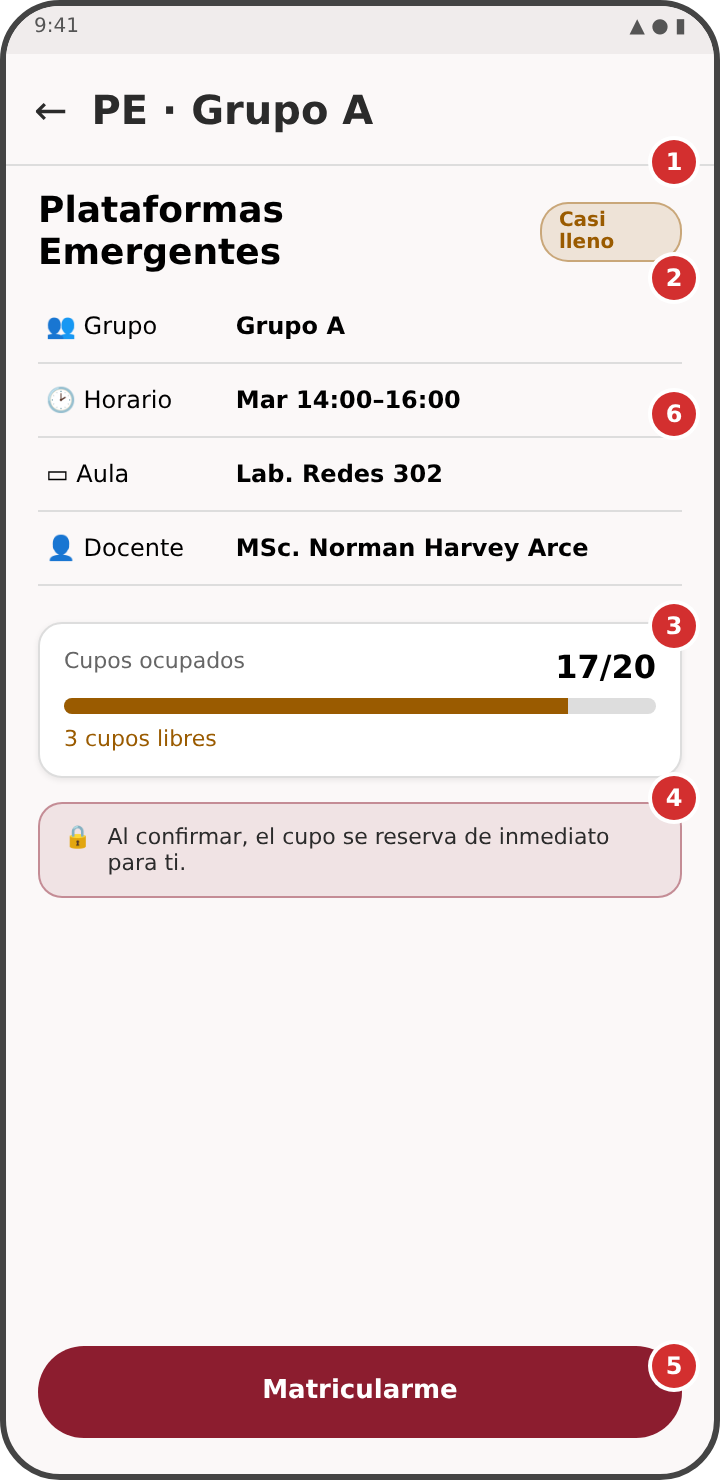
\includegraphics[width=\linewidth]{img/m04_grupo.png}\caption{Mockup}\end{subfigure}
\begin{subfigure}[t]{0.17\textwidth}\centering\capt{c06_grupo_detalle}{}\caption{App}\end{subfigure}\hfill
\begin{subfigure}[t]{0.17\textwidth}\centering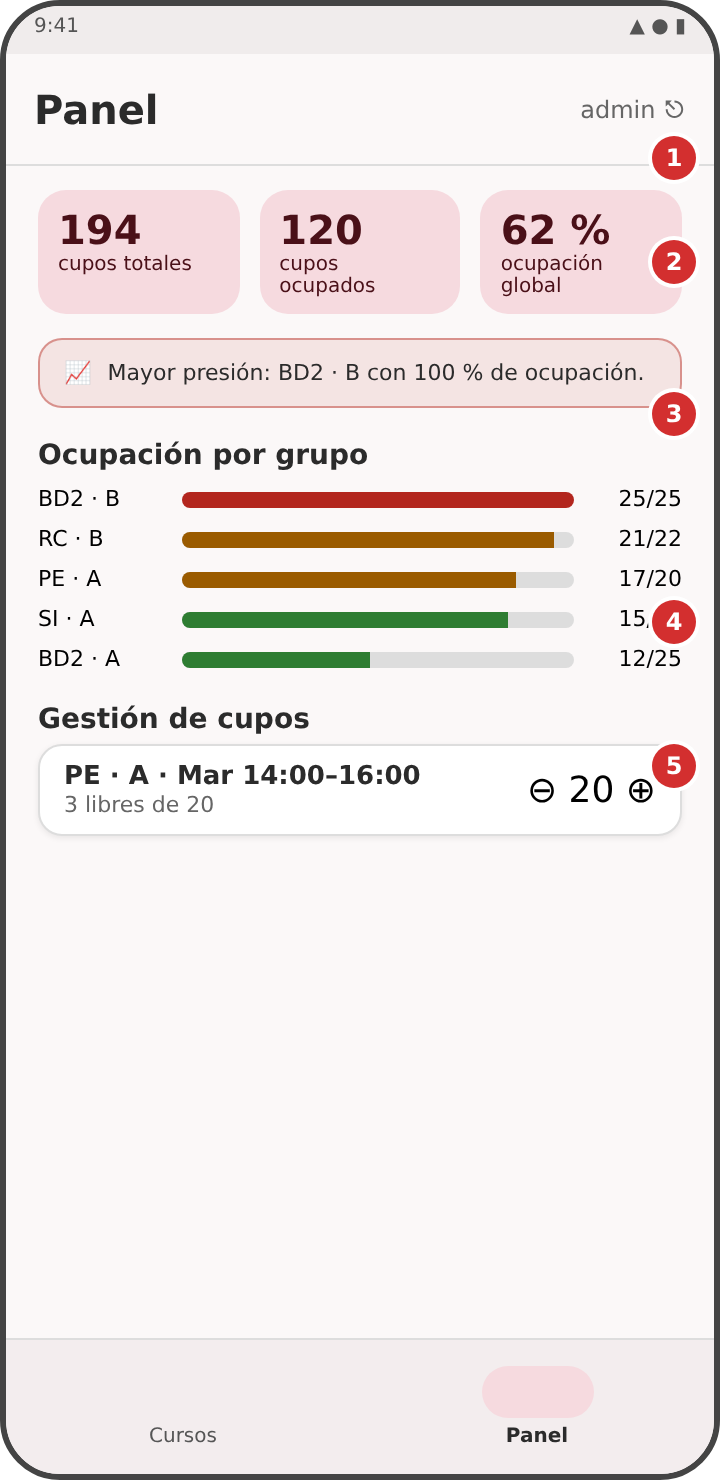
\includegraphics[width=\linewidth]{img/m09_panel.png}\caption{Mockup}\end{subfigure}
\begin{subfigure}[t]{0.17\textwidth}\centering\capt{c14_panel_admin}{}\caption{App}\end{subfigure}
\caption{Mockup frente a implementación: login, detalle de grupo y panel.}
\label{fig:comp}
\end{figure}

\subsection{Pruebas}
\label{sec:pruebas}
Escribí tres conjuntos de pruebas (carpeta \texttt{test/} del repositorio):
\begin{itemize}
	\item \textbf{Reglas de negocio} (\texttt{matrlab\_state\_test.dart}, 17 pruebas): validación de credenciales, matrícula con reserva de cupo, un solo grupo por curso, cruce de horario, grupo lleno, cancelación, lista de espera, notificación al agregar cupos, umbrales de estado, ranking y métricas, y solapamiento de horarios.
	\item \textbf{Flujo de interfaz} (\texttt{flujo\_widget\_test.dart}): login con validación, curso, grupo, hoja de confirmación, pantalla de éxito y horario, con widgets reales.
	\item \textbf{Capturas} (\texttt{capturas\_test.dart}): 17 pruebas que llevan la app a un punto del flujo y guardan una imagen en \texttt{capturas/}.
\end{itemize}

\pendiente{pegar aquí la salida de \texttt{flutter analyze} y \texttt{flutter test} ejecutados en el equipo del autor (por ejemplo, «All tests passed!» y el número de pruebas).}

\subsection{Registro de cambios}
Como pide la guía, los cambios sobre el trabajo se registran; en el código se marcan con comentarios \texttt{// CAMBIO:}.

\begin{table}[H]
	\centering\footnotesize
	\begin{tabularx}{\textwidth}{|p{1.4cm}|p{2.4cm}|X|}
		\hline
		\rowcolor{tablebackground}\color{white}\textbf{Versión} & \color{white}\textbf{Fecha} & \color{white}\textbf{Cambio}\\
		\hline
		1.0 & 24/10/2026 & Primera versión: investigación, mockups, aplicación Flutter de 9 pantallas, pruebas e informe. \\\hline
	\end{tabularx}
	\caption{Registro de cambios del trabajo.}
	\label{tab:cambios}
\end{table}
